
%%%%%%%%%%%%%%%%%%%%%%%%%%%%%%%%%%%%%%%%%%%%%%%%%%%%%%%%%%%%%%%%%%%%%%%%%%%
%
% Plantilla para un artculo en LaTeX en espaol.
%
%%%%%%%%%%%%%%%%%%%%%%%%%%%%%%%%%%%%%%%%%%%%%%%%%%%%%%%%%%%%%%%%%%%%%%%%%%%

\documentclass[11pt,twoside]{article}

% Esto es para poder escribir acentos directamente:
%\usepackage[latin1]{inputenc}
\usepackage[utf8]{inputenc}
\usepackage{makeidx}
\usepackage{multirow}
\usepackage{titlesec}
\usepackage{sectsty}
\usepackage{fncychap}

% Esto es para que el LaTeX sepa que el texto est en espaol:
\usepackage[spanish]{babel}
\usepackage[right=3cm,left=3cm,top=2.5cm,bottom=2.5cm,headsep=1cm,footskip=2cm]{geometry}
\usepackage{graphicx}
% Paquetes de la AMS:
\usepackage{amsmath, amsthm, amsfonts}

\usepackage{fancyhdr}
\pagestyle{fancy}
\lhead{
\chead{
\rhead{\bfseries Informe de Práctica }
%\lfoot{From: K. Grant}
%\cfoot{To: Dean A. Smith}
\rfoot{\thepage}
\renewcommand{\headrulewidth}{0.4pt}
\renewcommand{\footrulewidth}{0.4pt}
}}
\begin{document}
\setlength{\unitlength}{1 cm} %Especificar unidad de trabajo
\thispagestyle{empty}
\begin{picture}(0,1.5)
\put(0,0){
\includegraphics[width=2.7cm,height=2cm]{utfsm.jpg}}
\put(13,0){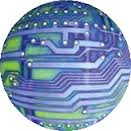
\includegraphics[width=2cm,height=2cm]{elo.jpg}}
\end{picture}
\\
\\
\begin{center}
\textbf{{\LARGE Universidad Técnica Federico Santa María}\\[0.5cm]
{\LARGE Departamento de Electrónica}}\\[4.25cm]
{\Large Informe de Práctica}\\[2.3cm]
{\LARGE \textbf{Centro Cient\'ifico Tecnol\'ogico de Valpara\'iso}}\\[3.5cm]
{\large Arturo Veras Olivos}\\[2cm]
Valparaiso - \today
\\
 {\large Versión 2.5}
\end{center}

%\newpage
%\tableofcontents
%\listoffigures % to produce list of figures
%\listoftables % to produce list of tables
\newpage
\section{Información General}

\subsection{Alumno}
\begin{tabular}{|l|l|}
\hline 
Nombre Completo: & Arturo Armando Veras Olivos \\ 
\hline 
Domicilio: & Garibaldi 205 - Cerro La Cruz, Valpara\'iso \\ 
\hline 
E-mail & a.veras@gmail.com \\ 
\hline 
Tel\'efono & +56 9 82413883 \\ 
\hline 
Rol USM: & 2521042-5 \\ 
\hline 
Carrera & Ingenier\'ia Civil Electr\'onica \\ 
\hline 
Curso: & Sexto año de la carrera \\ 
\hline 
Tipo de Pr\'actica & Profesional \\ 
\hline 
Fecha de inicio & 13/01/14 \\ 
\hline 
Fecha de t\'ermino & ??/03/14 \\ 
\hline 
Duraci\'on & 8 semanas \\ 
\hline 
\end{tabular} 
\subsection{Empresa}

\begin{tabular}{|l|l|}
\hline 
Nombre: & Centro Cient\'ifico Tecnologico de Valpara\'iso \\ 
\hline 
Direcci\'on: & Avenida España 1680, Valpara\'iso \\ 
\hline 
RUT:  & 81.668.700-4 \\ 
\hline 
Direcci\'on Web: & www.cctval.cl \\ 
\hline 
\end{tabular} 

\subsection{Supervisor}
\begin{tabular}{|l|l|}
\hline 
Nombre: & Claudio Torres \\ 
\hline 
Cargo: &   \\ 
\hline 
Oficio o profesi\'on:  & 81.668.700-4 \\ 
\hline 
Tel\'efono: & +56 (32) 2654418 \\ 
\hline 
E-mail: & ctorres@inf.utfsm.cl \\ 
\hline
\end{tabular} 

\section{Resumen Ejecutivo}

Las evaluaciones que se realizaran tendrán que ver con el funcionamiento correcto, el desempeño y la puesta en practica. Lo primera evaluación sera verificar el correcto flujo de datos entre módulos, es decir, que los datos esperados para crear serie de movimientos sean los correctos. Luego realizaran pruebas sobre el funcionamiento del modulo, esto quiere decir que se deberá utilizar algún simulador para que facilite las pruebas y asegure que el modulo entrega los resultados que se esperados. Por último se evaluara la rapidez de respuesta del modulo, en este tipo de navegación se espera que el robot responda rápidamente a nuevos a los distintos tipos de escenarios por lo que es imprescindible que modulo sea capaz de responder rápidamente.

\section{Actividad del Lugar de Trabajo}
Los resultados esperados tienen directa relación con la evaluación, es decir , se espera que el modulo a desarrollar genere un sistema de navegación eficiente que responda a las demandas de movilidad dentro múltiples escenarios.

\section{Organigrama de la Empresa}

\section{Preparaci\'on de la pr\'actica}

\section{Sugerencia de Proyecto Innovador}

\end{document}
